\documentclass[czech,bachelor]{diploma}

\usepackage[autostyle=true,czech=quotes]{csquotes}
\usepackage[backend=biber, style=iso-numeric, alldates=iso]{biblatex}
\usepackage{dcolumn}
\usepackage{subfig}
\usepackage[cpp]{diplomalst}

\addbibresource{biblatex.bib}

\ThesisAuthor{Ratmir Gaitov}
\ThesisSupervisor{Ing. Petr Olivka, Ph.D.}
\CzechThesisTitle{Autonomní řízení auto - optimalizace řízení dle pohybových senzorů}
\EnglishThesisTitle{Autonomous Car Control - Speed Optimization According to Motion Sensors}
\SubmissionYear{2024}
\ThesisAssignmentFileName{ThesisAssignment.pdf}

\Acknowledgement{Rád bych na tomto místě poděkoval mého vědoucího Petra Olivku, který mi s prací pomohl, protože bez nich by tato práce nevznikla.}

\CzechAbstract{
Tato práce popisuje ovládání modelu automobilu používaného na mezinárodní soutěží NXP Cup, konkretně korigování rychlosti jízdy pomocí pohybových senzorů.
Jsou provedeny testy různých senzoru a signálových filtru, ze kterých pak vybraná nejlepší konfigurace.
Tyto vybrané signálové filtry pak implementovaný v kombinace se vhodnými senzory.
}
\CzechKeywords{Automatické regulování rychlosti; Signálové filtry; NXP Cup; FRDM-K66F}

\EnglishAbstract{This paper describes the control of a model car used in the international NXP Cup competition, specifically the correction of driving speed using motion sensors.
Tests of different sensor and signal filters are performed, from which the best configuration is then selected.
These selected signal filters are then implemented in combination with suitable sensors.}
\EnglishKeywords{Automatic speed control; Signal filters; NXP Cup; FRDM-K66F}

\AddAcronym{ARM}{Advanced RISC Machine}
\AddAcronym{GPIO}{General-Purpose Input/Output}
\AddAcronym{IMU}{Inertial Measurement Unit}
\AddAcronym{LED}{Light-Emitting Diode}
\AddAcronym{MCU}{Micro Controller Unit}
\AddAcronym{MEMS}{Micro-Electro-Mechanical System}
\AddAcronym{NiMH}{Nickel-Metal Hydride}
\AddAcronym{PWM}{Pulse Width Modulation}
\AddAcronym{RAM}{Random Access Memory}
\AddAcronym{SDHC}{Secure Digital High Capacity}
\AddAcronym{WiFi}{Wireless Fidelity}
\AddAcronym{$I^2C$}{Inter-Integrated Circuit}
\AddAcronym{UDP}{User Datagram Protocol}
\AddAcronym{JSON}{JavaScript Object Notation}
\AddAcronym{PNG}{Portable Network Graphics}
\AddAcronym{RC}{Remote control}

\newcolumntype{d}[1]{D{,}{,}{#1}}
\renewcommand{\lstlistlistingname}{Seznam výpisů zdrojového kódu}
\renewcommand{\lstlistingname}{Výpis}

\begin{document}
\MakeTitlePages

\listoffigures
\clearpage

\listoftables
\clearpage

\lstlistoflistings
\addcontentsline{toc}{chapter}{\lstlistlistingname}
\clearpage

\chapter*{Úvod}
\label{sec:Introduction}
\addcontentsline{toc}{chapter}{\protect\numberline{}Úvod}\

Autonomní řízení automobilů je v~současné době velmi populárním tématem, přičemž
výrobci automobilů se předhánějí o~prvenství v~této oblasti. Jedná se především
o~velmi komplexní oblast, kde musí být správně vyřešeny všechny možné situace, jelikož
jakýkoliv přehlédnutý detail může způsobit újmu na zdraví. Z~tohoto důvodu je
autonomní řízení částí populace stále vnímáno jako něco  nepřijatelného, ovšem
zvyšující se rychlost vývoje naznačuje, že v~následujících letech dojde k~významnému
pokroku v~této oblasti a~setkávání autonomně řízenými auty bude běžným jevem.

V~této bakalářské práci bude popsán způsob automatického řízení auta a~korekce 
rychlosti na základě informací z~pohybových senzorů. Práce začne popisem modelu 
automobilu pro testování. Následně budou popsány algoritmy pro automatické a~manuální 
řízení. Další část se bude zabývat metodami pro zobrazování a~ukládání hodnot dat auta 
během jízdy. Poté budou otestovány a~vybrány vhodné senzory a~filtry pro detekci fáze 
jízdy. V~závěrečné části práce bude popsán algoritmus pro optimalizaci rychlosti 
a~provedeno porovnání s~manuálním řízením.

\endinput
\chapter{Model automobilu}
\label{sec:CarModel}\

V~této kapitole je popsán model automobilu a~jeho jednotlivé součásti.

Model automobilu je založen na podvozku typu Alamak, která má \textbf{1 servomotor}
pro řízení a~\textbf{2 motory} pro pohon. \textbf{Podvozek Alamak} je řízen pomocí 
\textbf{NXP Freedom K66F} spolu s~modulem \textbf{POLI-TFC} 
přípojeným do GPIO pinů MCU. Detailní popis MCU a~modulu jsou v~podkapitolách 
\ref{sec:FRDM-K66F} a~\ref{sec:POLI-TFC}.

Pro manuální řízení je zapojen přijímač RC signálu \textbf{Minima 6S} do pinu
POLI-TFC shieldu. Přijímač pak přijímá signály z~vysílače \textbf{Hitec OPTIC 6 
SPORT}.

Pro komunikaci s~podvozkem Alamak je použit \textbf{WiFi Access Point}, který je
připojen k~MCU pomocí Ethernet portu. \textbf{Řádková kamera}, která je umístěna
v~přední části, se používá pro získání obrazu dráhy. Všechny součástky
jsou napájeny baterií typu \textbf{NiMH} o~napětí 7,2 V.

Celý model je zobrazen na obrázku \ref{fig:car}.
\begin{figure}[!h]
    \centering
    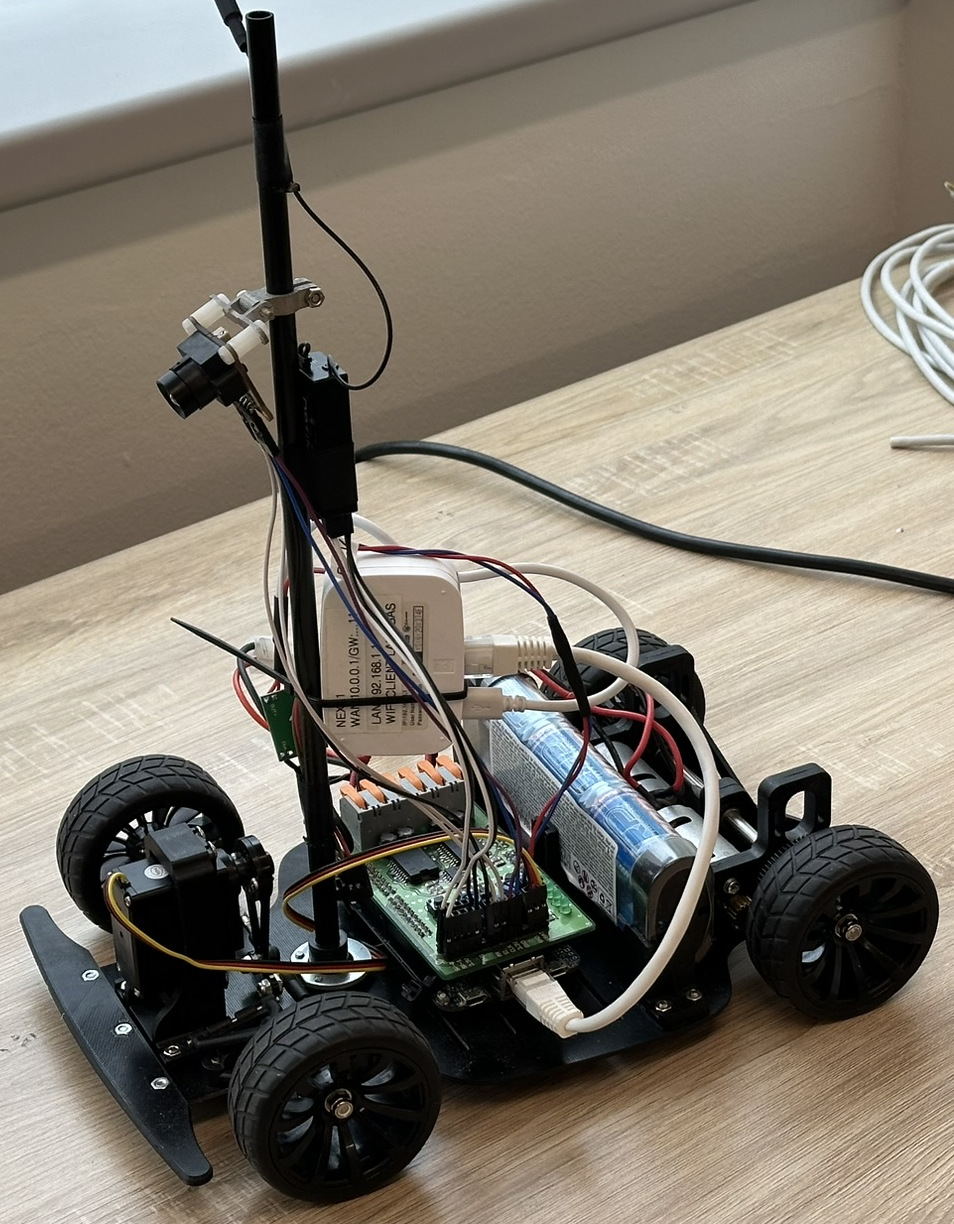
\includegraphics[width = .4\linewidth]{Figures/Car.jpeg}
    \caption{Model auta.}
    \label{fig:car}
\end{figure}

\section{FRDM-K66F}
\label{sec:FRDM-K66F}\

\textbf{FRDM-K66F} je vývojová platforma od společnosti NXP určená pro MCU řady 
Kinetis K66 a~K26. Platforma je založena na jádře \textbf{ARM© Cortex®-M4}
a~využívá model \textbf{MK66FN2M0VMD18} s~frekvencí 180 MHz, 2 MB flash paměti
a~256 KB RAM \cite{frdmk66UserGuide}.

Konektivitu zajišťují 2 micro-B USB porty, 1 ethernetový port a~54 GPIO pinů.
GPIO~piny jsou kompatibilní s~\textbf{Arduino™ R3}, čímž je poskytnuta široká škála
možností pro rozšiřující desky. Deska umožňuje bezdrátové možností konektivity
pomocí modulů Bluetooth a~RF \cite{frdmk66UserGuide}.

Pro ladění je na platformě přítomno rozhraní \textbf{OpenSDAv2.1}, které podporuje
J-Link. J-Link~je sériový programovací adaptér, který umožňuje programování
a~debugování mikrokontrolérů \cite{frdmk66UserGuide}.

Další užitečné periferie na desce zahrnují trojbarevnou LED, SDHC a~digitální MEMS
mikrofon~\cite{frdmk66UserGuide}.

Jako \textbf{inerciální měřicí jednotku} (IMU) platforma využívá akcelerometr
společně s~magnetometrem a~gyroskopem \cite{frdmk66UserGuide}.

Vývojová platforma je znázorněna na obrázku \ref{fig:FRDM-K66F}.

\section{POLI-TFC}
\label{sec:POLI-TFC}\

\textbf{POLI-TFC shield} je rozšiřující deska pro FRDM-K66F, která rozšiřuje
rozhraní pro připojení periferií k~vývojové desce. Shield obsahuje 2 konektory
pro motory, 2 servomotory, 2 rozhraní pro~připojení řádkových kamer, 2 
potenciometry, 4 DIP přepínače a~4 LED diody. 

Shield~je zobrazen na obrázku \ref{fig:POLI-TFC}.

\begin{figure}[h]
    \begin{subfigure}{0.45\textwidth}
        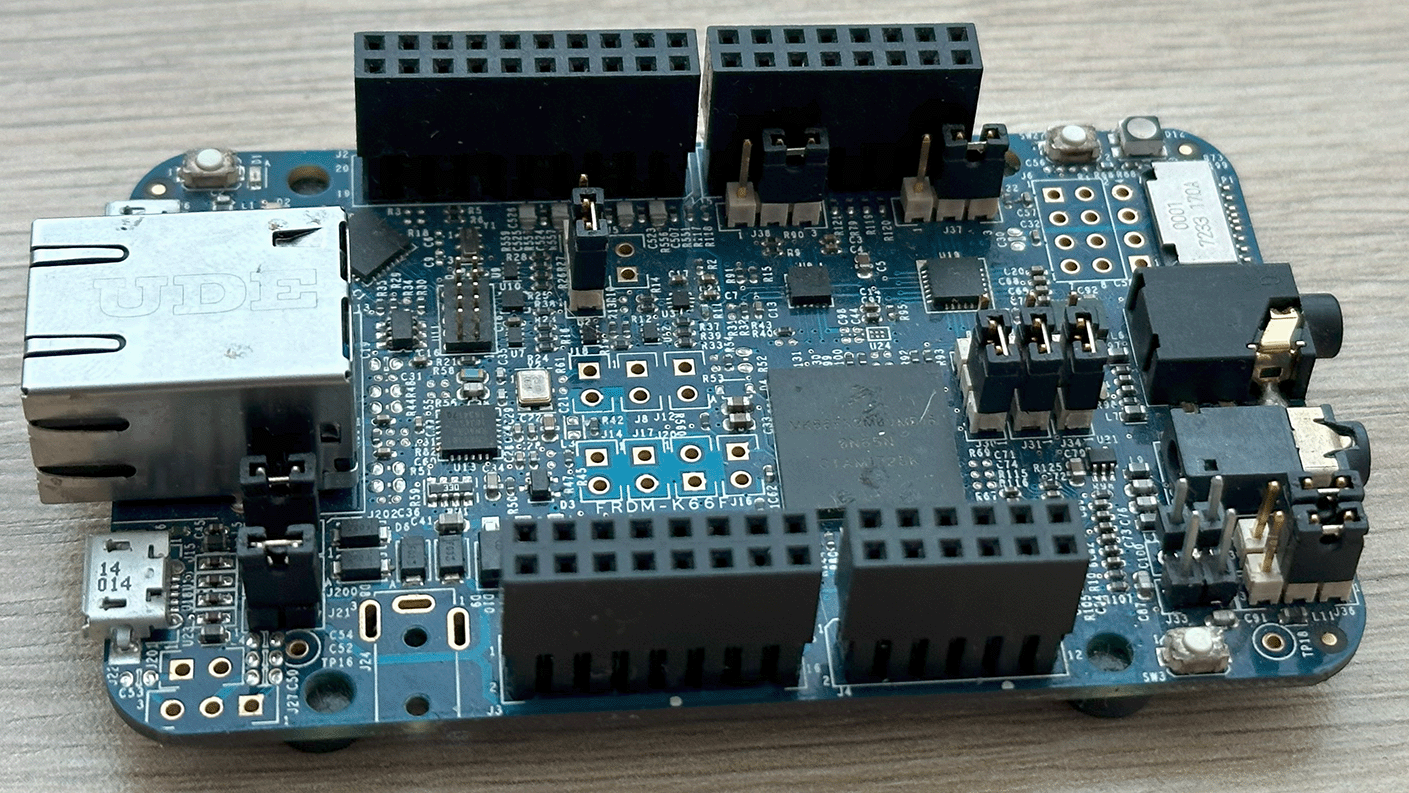
\includegraphics[width=\textwidth, height = 5cm]{Figures/FRDM-K66F.png} 
        \caption{FRDM-K66F.}
        \label{fig:FRDM-K66F}
    \end{subfigure}
    \hfill
    \begin{subfigure}{0.45\textwidth}
    	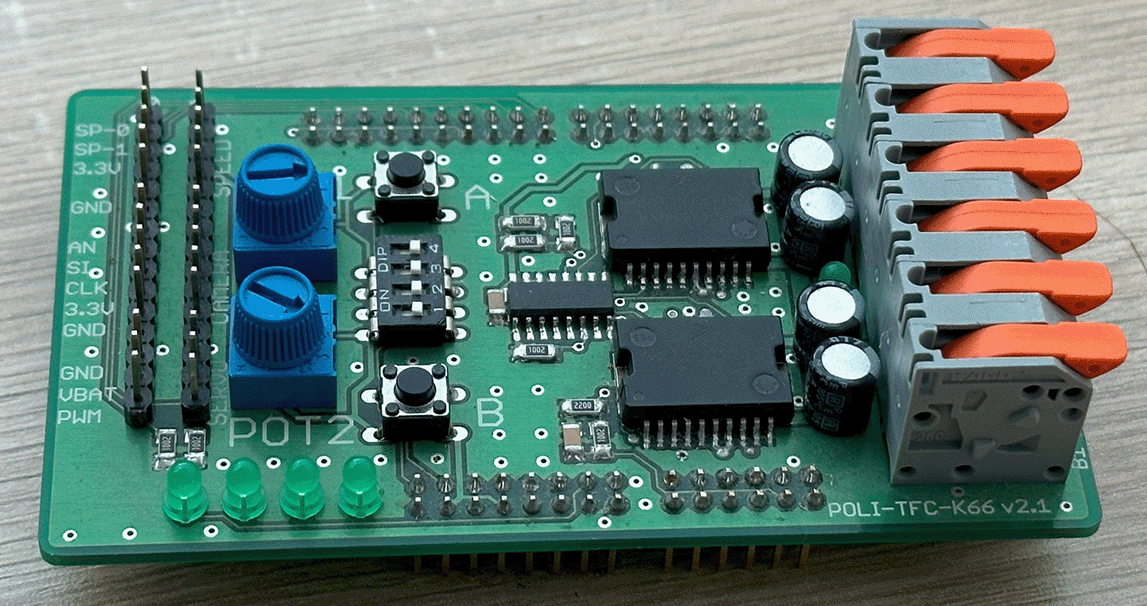
\includegraphics[width=\textwidth, height = 5cm]{Figures/POLI-TFC.png}
    	\caption{POLI-TFC.}
    	\label{fig:POLI-TFC}
	\end{subfigure}
    \caption{Vývojová platforma FRDM-K66F a~POLI-TFC shield.}
\end{figure}

\endinput
\chapter{Současný stav řešené problematiky}
\label{sec:Theory}\

V této kapitole bude popsán stav problematiky automatického řízení a pohybových
senzorů. Konkretně bude popsaná práce \uv{Krokoměr s mikropočítačem ARM}\cite{krokomer} Šigurda Filipa, který používá ve své práce akcelerometry. Následné
budou popsaný práci \uv{Autonomní řízení auta - optimalizace detekce dráhy}\cite{draha} i \uv{Mechanizmy řízení robotického auta NXP (FREESCALE)}\cite{robot},
které popisuje autonomní řízení na základe řádkové kamery a senzorů. Autoři jsou
Vojtěch Ihn a Richard Zvonek.

\section{Krokoměr s mikropočítačem ARM}\

Tato práce se zabývala vývojem krokoměru s využitím desky NXP FRDM-K64F, která je
založená na jádře ARM© Cortex®-M4. Hlavním cílem práce bylo vytvoření krokoměru,
který by byl schopen detekovat a počítat kroky uživatele.

V práci byly vybírány různé MEMS akcelerometry podle několika kritérií: možnosti
integrace na plošný spoj, cenové dostupnosti, schopnosti komunikovat s
mikrokontrolérem prostřednictvím rozhraní $I^2C$ nebo SPI, přičemž byly vybírány
výhradně tříosé akcelerometry.

Akcelerometry byly následně testovány v různých prostředích a podmínkách, které
zahrnovaly chůzi po~rovině, po trávě, do a z kopce, a také chůzi do a ze schodů.

Každé měření bylo doprovázeno dvěma krokoměry:  Xiaomi Mi Band a aplikace
\uv{Pedometer} provozovanou na mobilním telefonu Nokia 6.1. Výsledky jednotlivých
akcelerometrů v~jednotlivých situacích byli velice podobné:

\begin{table}[!h]
	\centering
	\begin{tabular}{lccc}
		\toprule
		Měření s akcelerometrem      & délka chůze & Xiaomi Mi Band & Nokia 6.1 \\
		\midrule
		NXP FXOS8700CQ               & 3m 35s      & 345            & 351       \\
		NXP MMA8452Q                 & 3m 25s      & 339            & 337       \\
		Analog Devices ADXL345       & 3m 31s      & 343            & 339       \\
		STMicroelectronics LSM303DLH & 3m 30s      & 338            & 336       \\
		\bottomrule
	\end{tabular}
	\caption{Počet kroků při chůzi do kopce s krokoměrem v ruce\cite{krokomer}.}
	\label{tab:1}
\end{table}

Dále byly otestovány a porovnány různé filtry pro odstranění šumu z naměřených dat.
Použity byly filtry typu dolní propust, a to z důvodu, že normální chůze
nepřekračuje rychlost čtyř kroků za~sekundu, což znamená, že frekvence vyšší než
4~Hz byly považovány za šum. Filtrace signálu byla prováděna pomoci filtrů s
konečnou impulzní odezvou (FIR) a s nekonečnou impulzní odezvou~(IIR).

\begin{figure}[!h]
	\centering
	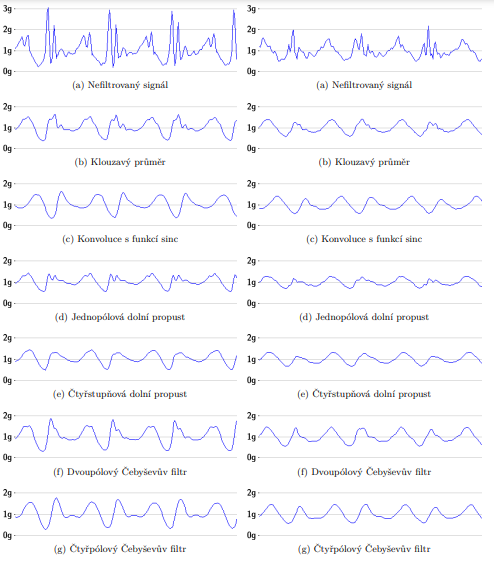
\includegraphics[width = .95\linewidth]{Figures/Filtry.png}
	\captionsetup{justification = centering}
	\caption{Čtyřsekundové ukázky aplikovaných filtrů. Vlevo: chůze po rovině s
	akcelerometrem v~kapse. Vpravo: chůze do kopce s akcelerometrem v
	kapse\cite{krokomer}.}
	\label{fig:filtr}
\end{figure}

Po porovnání filtrů byl jako nejlepší vyhodnocen dvoupólový Čebyševův filtr, který
ve srovnání s ostatními je výpočetně méně náročný a odstranil velké množství šumu se
zachováním amplitudy signálu. Výsledky aplikace filtrů jsou zobrazeny na obrázku \ref{fig:filtr}.

Pro počítání kroků byly implementovány dva způsoby detekce kroků. První z nich se
ukázal jako nevyhovující. Druhý způsob detekce kroků byl o poznáni přesnější.
Algoritmus funguje na principu stavového automatu, který má 2 stavy pro hledání
nástupních a sestupných hran.

Závěrečné testování kompletního řešení proběhlo chůzi po městě. Trasa byla přibližně
1650~metrů dlouhá. Výsledky měření byly porovnány s komerčně dostupnými krokoměry
pro ověření přesnosti navrženého řešení. Tabulka \ref{tab:2}  zobrazuje počty
naměřených kroků jednotlivými krokoměry.

Testování ukázalo, že výsledky jsou velmi podobné výsledkům ostatních dvou
krokoměrů\cite{krokomer}.

\begin{table}[!h]
	\centering
	\begin{tabular}{lcccc}
		\toprule
		Umístění krokoměru & délka chůze & Xiaomi Mi Band & Nokia 6.1 & FRDM-K64F \\
		\midrule
		V kapse            & 18m 46s     & 1986           & 2013      & 2021      \\
		V ruce             & 18m 36s     & 1993           & 2007      & 2010      \\
		\bottomrule
	\end{tabular}
	\caption{Počet kroků při závěrečném měření\cite{krokomer}.}
	\label{tab:2}
	\vspace{-10pt}
\end{table}

\section{Autonomní řízení auta - optimalizace detekce dráhy}\

Tato práce se zaměřila na zpracování obrazu získaného z řádkové kamery a na následné
vyhledávání okrajových čar dráhy s využitím různých typů objektivů a filtrů. Cílem
bylo najít optimální kombinaci, která by umožňovala nejpřesnější detekci dráhy pro
autonomní řízení vozidla. Pro dosažení tohoto cíle práce zkoumala různé metody a
techniky zpracování obrazu, včetně výběru a testování objektivů kamery, aplikaci
filtrů pro zlepšení kvality obrazu a implementaci algoritmů pro~efektivní detekci
dráhy.

Finální výběr kamery a objektivu byl založen na schopnosti kamer efektivně detekovat
okrajové čáry za různých světelných podmínek.

Dále byly otestovány různé kombinace filtrů pro redukci šumu, detekci hran a
prahování. Ve~výsledku byly pro implementaci vybrány 4 filtry: mediánový filtr,
Gaussův filtr, morfologický gradient a Otsu prahování.

Algoritmus byl testován při umělém osvětlení i při denním světle. Při rovnoměrném
umělém osvětlení byla detekce okrajových čar na dráze spolehlivá. Při denním světle
byly dosaženy slušné výsledky, které avšak nešlo považovat za ideální\cite{draha}.

\section{Mechanizmy řízení robotického auta NXP (FREESCALE)}\

V rámci této práce byl vyvinut softwarový systém pro robotický model auta. Systém
byl navržen tak, aby umožňoval autonomní navigaci po závodní dráze s využitím dat
získaných z řádkové kamery a dalších senzorů. Řídící software se skládal ze dvou
hlavních částí: zpracování obrazu z řádkové kamery a řízení na základě získaných
informací z obrazu.

Pro zpracování obrazu byly použitý: filtrování mediánem pro odstranění šumu,
normalizace obrazu pro přizpůsobení světelným podmínkám a prahování průměrem.

Pro řízení pomocí dat z kamery byl software schopen detekovat okraje dráhy a na
základě této informace řídit směr a rychlost auta. Klíčovým prvkem bylo efektivní
využití PID regulátoru.

Práce rovněž zahrnovala vývoj a integraci různých senzorů, včetně IMU a IR senzorů.
IMU~jednotka byla použita k detekci zastavení vozidla, zatímco infračervené senzory
sloužily k detekci blízkých objektů a překážek.

Následně bylo robotické auto testováno na soutěži NXP Cup, kde úspěšně zvládlo
všechny tři dodatečné disciplíny v kvalifikačním kole\cite{robot}.

\endinput

\chapter{Komunikace s~modelem auta}
\label{sec:PlatformCommunication}\

V~této kapitole je popsán způsob zobrazení a~ukládání dat během jízdy.

Během jízdy je důležité posílat data asynchronně, aby nebyl blokován hlavní
algoritmus auta. Z~toho důvodu pro komunikaci s~platformou je použit \textbf{UDP}
(User Datagram Protocol) protokol, který se primárně používá pro časově citlivé
informace. Zrychluje komunikaci tím, že před přenosem dat není nutné formálně
navazovat spojení, což umožňuje velmi rychlý přenos dat \cite{UDP}.

Během komunikace se vývojová deska chová jako UDP server a~klient pro server je
aplikací sloužící k~zobrazení dat. Aplikace pro zobrazení dat byla pojmenována jako
CarQt. \textbf{CarQt} umí zobrazovat originální obraz, normalizovány obraz
a~prahovaný obraz. Informace o~Regionech, PWM~motorech, servo motorech a~senzorech
jsou zobrazeny v~číselném formátu. Ukládání číselných dat je implementováno ve
formátu \textbf{JSON} (JavaScript Object Notation) a~originálního obrazu ve formátu
\textbf{PNG}~(Portable Network Graphics) souboru. Ukládaní do formátu JSON je napsáno pomocí knihovny JsonCpp. CarQt je napsána pomocí knihoven
Qt, JsonCpp a~OpenCV. Aplikace je zobrazena na obrázku \ref{fig:CarQt}.

\begin{figure}[!h]
    \centering
    \vspace{-10pt}
    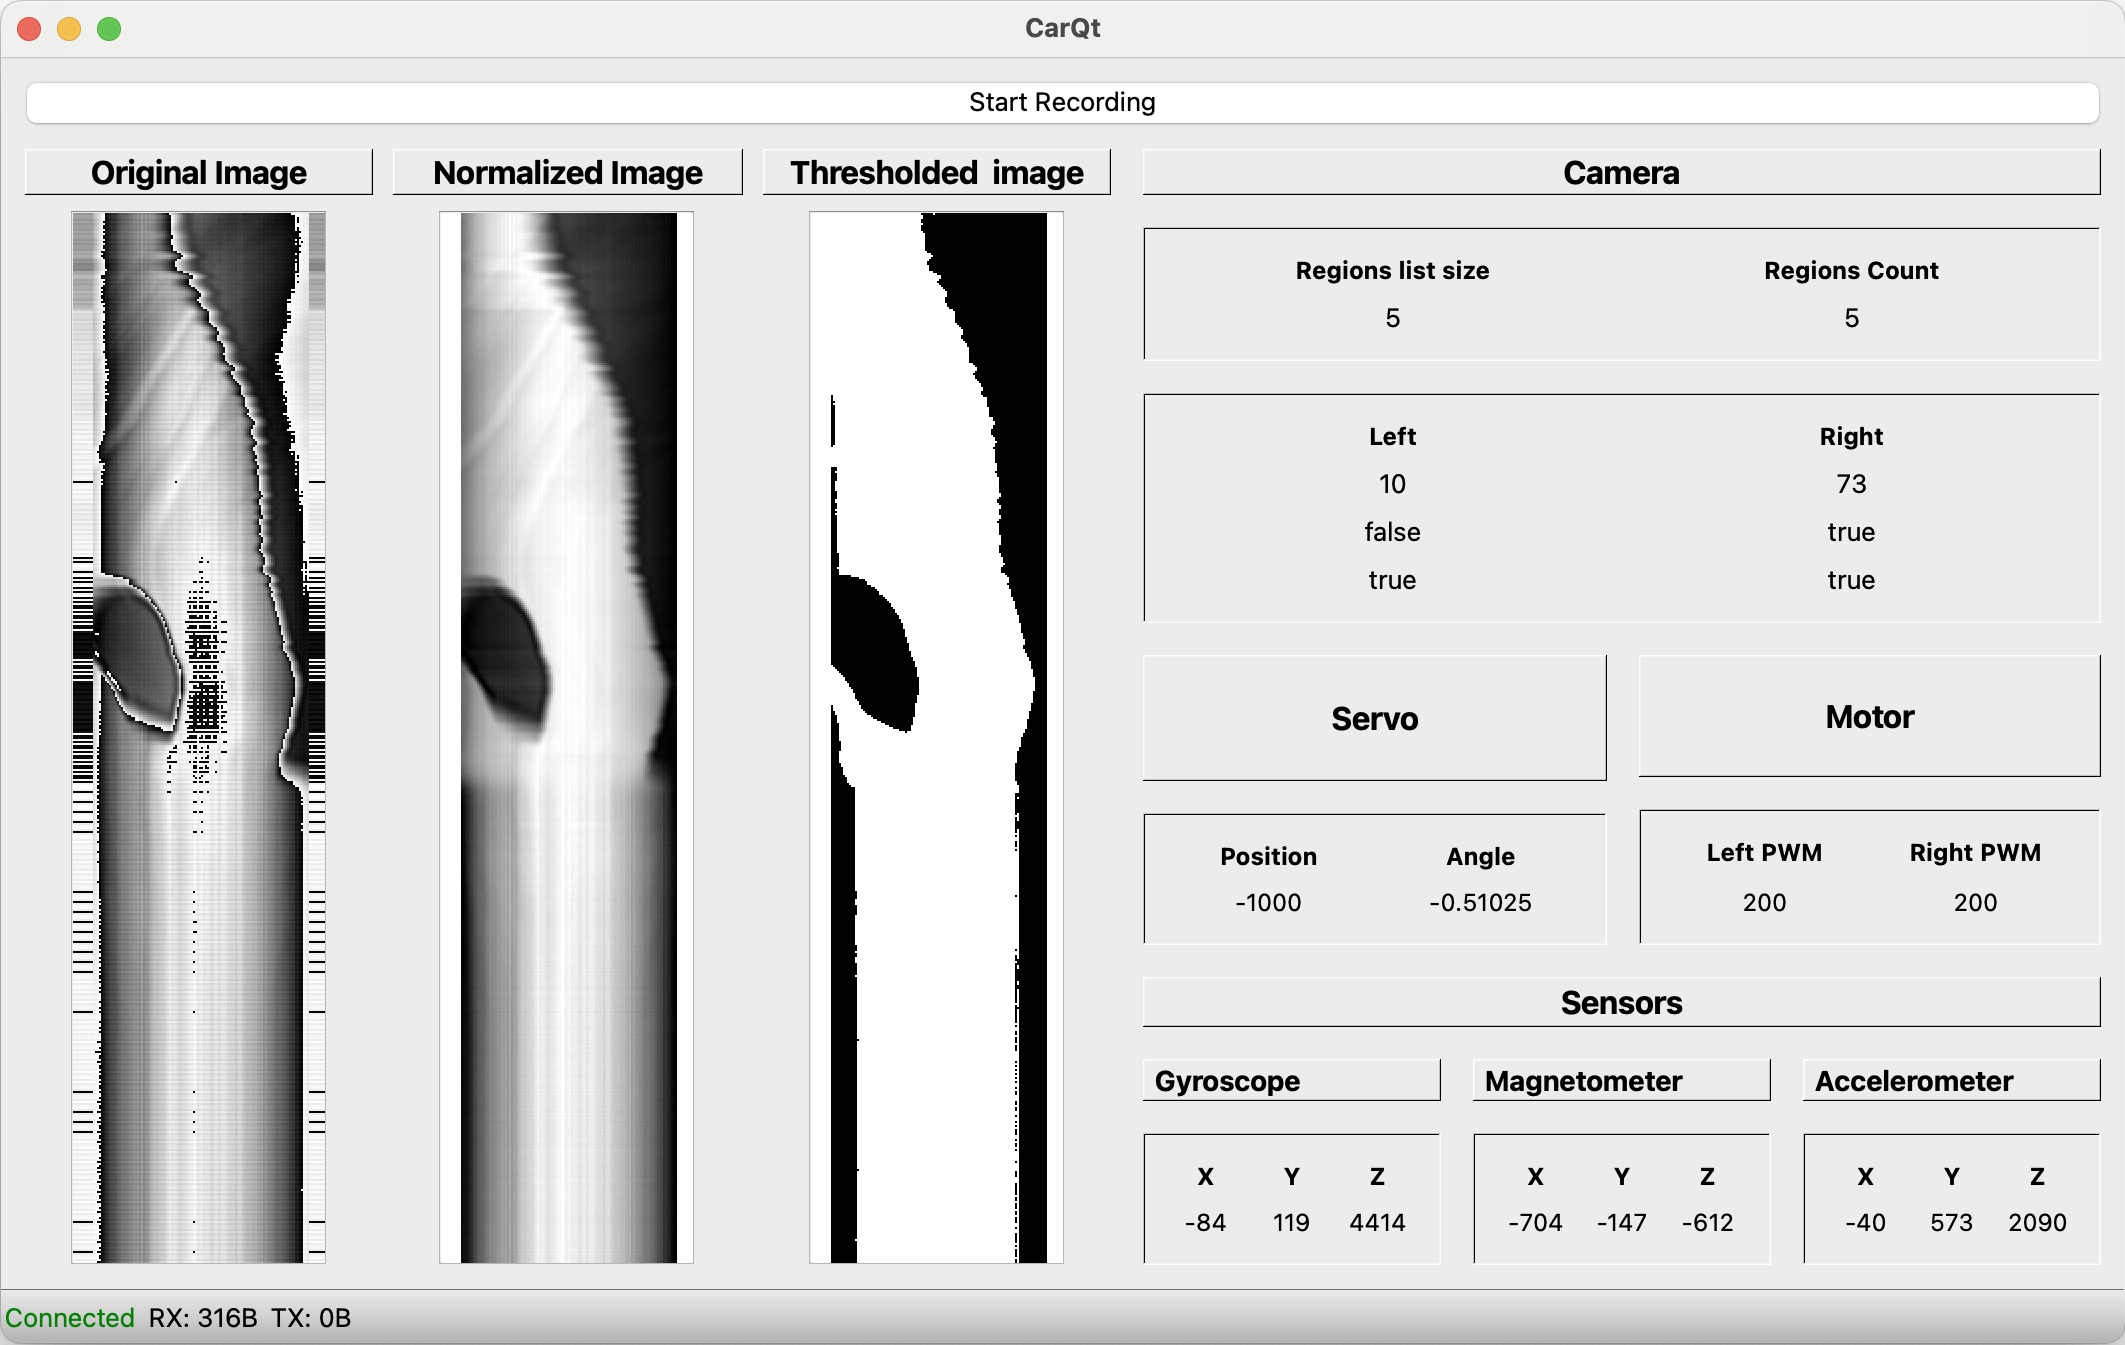
\includegraphics[width = .8\linewidth]{Figures/CarQt.png}
    \caption{CarQt aplikace.}
    \label{fig:CarQt}
    \vspace{-15pt}
\end{figure}

Pro přenos a~ukládání dat je použita struktura \textbf{Data}, která obsahuje:
\begin{itemize}
    \item originální data z~kamery,
    \item distance do levé i~pravé černé čáry,
    \item PWM hodnoty motorů,
    \item pozice a~úhel servomotoru,
    \item orientace senzorů,
    \item počet regionů.
\end{itemize}

Popis regionu je v~podkapitole \ref{sec:servocontrol}.
Implementovaná struktura Data je ve výpisu \ref{lst:data}.
\begin{lstlisting}[caption = Struktura Data., label = lst:data]
struct Data {
    uint16_t line[Image::LINE_LENGTH] = {0};
    uint32_t regionsCount = 0;
    uint32_t regionsListSize = 0;
    bool unchangedLeft = false;
    bool unchangedRight = false;
    bool hasLeft = false;
    bool hasRight = false;
    uint8_t leftDistance = 0;
    uint8_t rightDistance = 0;
    int32_t leftSpeed = 0;
    int32_t rightSpeed = 0;
    int32_t servoPosition = 0;
    float angle = .0f;
    Vec3<int16_t> accel = {0, 0, 0};
    Vec3<int16_t> mag = {0, 0, 0};
    Vec3<int16_t> gyro = {0, 0, 0};
    uint32_t timestamp = 0;
    uint8_t mode = Mode::None;
};
\end{lstlisting}

Na základě testování bylo nutné nastavit síťové adresy pro přenos dat. V~aplikaci je tak možné specifikovat konkrétní IP adresy, port a~cestu pro ukládání dat. Toto nastavení se ukládá ve formátu JSON. Okno nastavení je zobrazeno na obrázku \ref{fig:CarQtSettings}.
\begin{figure}[!h]
\centering
    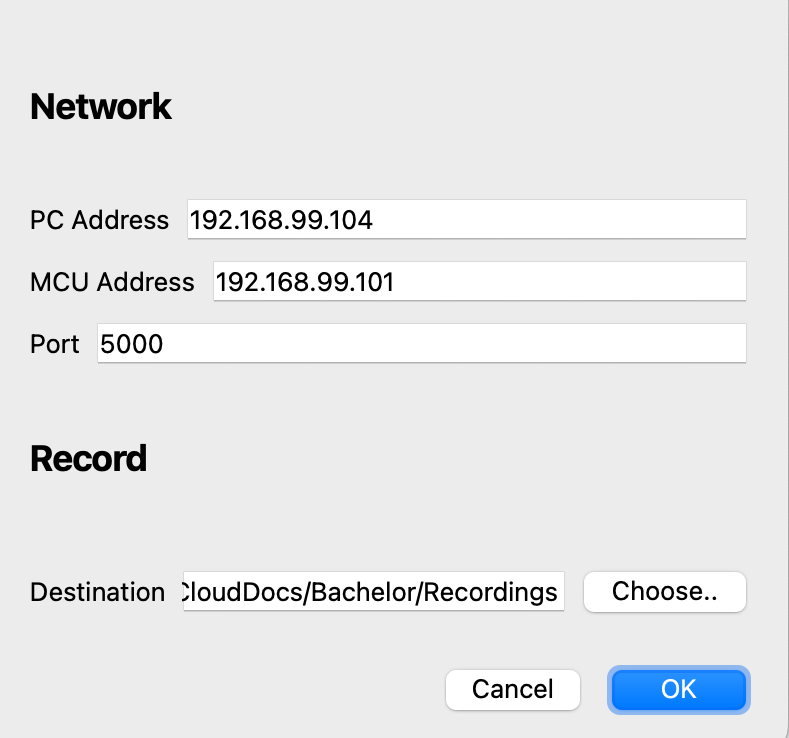
\includegraphics[width = .5\linewidth]{Figures/SettingsWindow.png}
\caption{Nastávení aplikace CarQt.}
\label{fig:CarQtSettings}
\end{figure}

\endinput
\chapter{Řízení modelu auta}
\label{sec:PlatformControl}\

V~této kapitole je popsán způsob manuálního a~automatického řízení. Pro automatické
řízení je popsán způsob rozpoznání dráhy a~řízení servo i~motorů. Pro manuální
řízení je popsán způsob ovládaní auta pomocí RC ovladače. Přepínáni mezi režimy
bylo implementováno pomocí tlačítka A~na POLI-TFC.


\section{Dráha}\

Testování řízení platformy bylo provedeno na dráze ve tvaru čísla 8.

Dráha je zobrazena na obrázku \ref{fig:Road}.

\begin{figure}[!h]
    \centering
    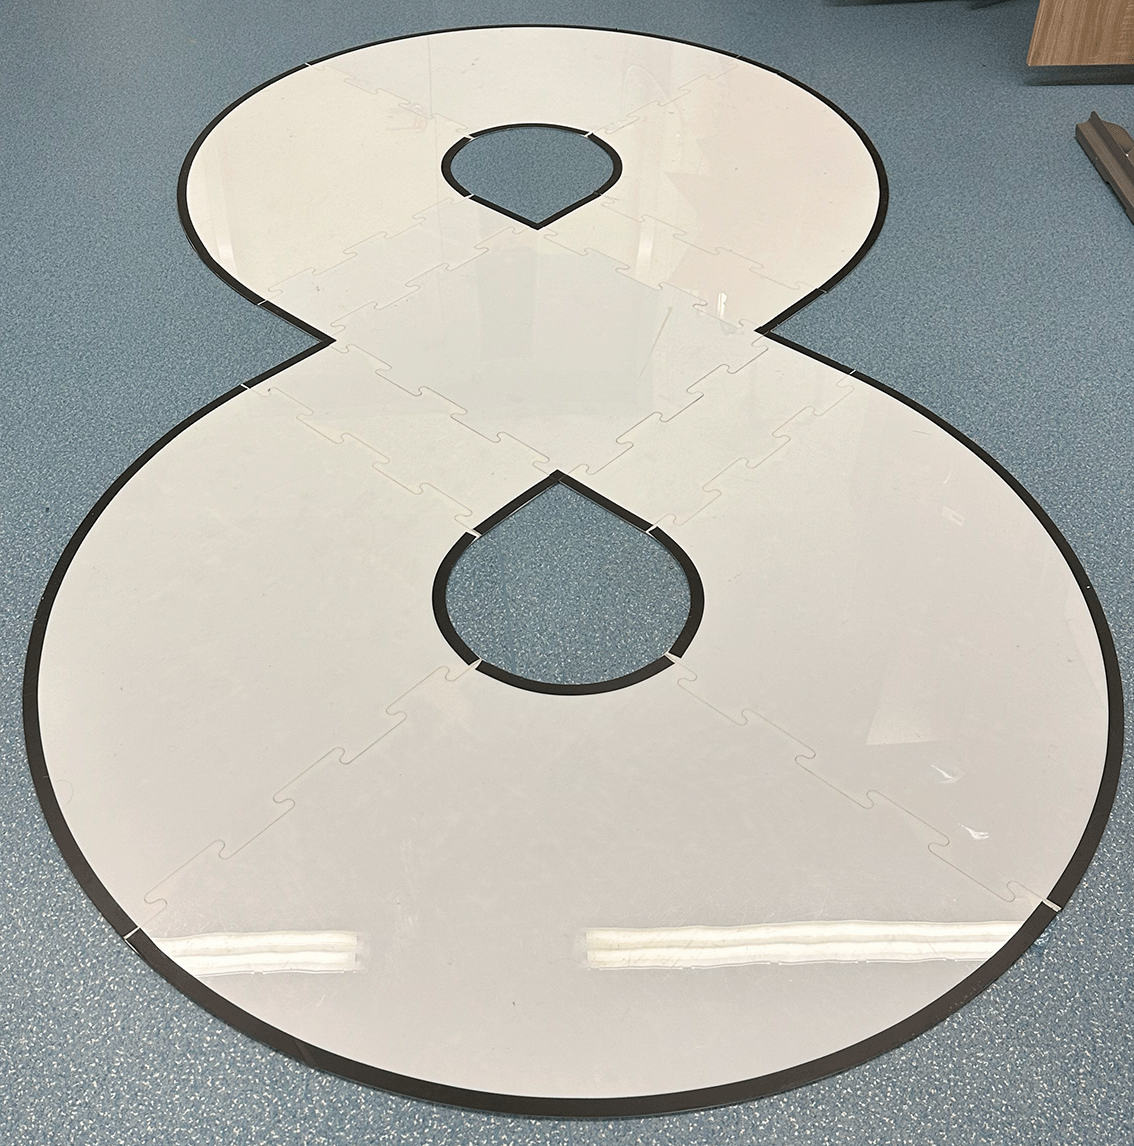
\includegraphics[width = .55\linewidth]{Figures/Road.png}
    \caption{Dráha.}
    \label{fig:Road}
    \vspace{-15pt}
\end{figure}

\section{Automatické řízení}\

\textbf{Automatické řízení} se skládá ze dvou častí. První je algoritmus rozpoznání 
drahý pomocí řádkové kamery. Druhá je kontrola motoru a~servo na základě těchto dat. 
Implementace řízení je inspirovaná bakalářskou práce Zvonka Richarda \uv{Mechanizmy 
řízení robotického auta NXP (FREESCALE)} \cite{robot}.

\subsection{Rozpoznání dráhy}\

Nejprve bylo zapotřebí získat obraz, který zajišťuje řádková kamera. Pro formát dat
je použita třída TFC \cite{draha}, která vrací data ve formátu 1D pole typu 
uint16\_t (16bitové celá čísla bez znaménka) v~intervalu <0; 4095>.

Obraz se zpracovává v~následujících krocích:
\begin{enumerate}
    \item Filtrování mediánem;
    \item Normalizace obrazu;
    \item Prahování průměrem.
\end{enumerate}

\subsubsection*{Filtrování mediánem}\

\textbf{Filtrování mediánem} je užitečné pro odstranění malých artefaktů v~obraze.
Zpracování pixelů probíhá na základě jeho okolních pixelů. Je zapotřebí tak mít
uloženy všechny pixely. Každá hodnota pixelu je nahrazena mediánem hodnot v~určitém
okolí daného pixelu, což pomáhá zachovat ostré hrany obrazu, zatímco šum je
redukován. Ukázka použitého algoritmu je ve výpisu \ref{lst:slowMedianBlur} 
\cite{draha}\cite{robot}.

\begin{lstlisting}[caption = Filtrování mediánem., label = lst:slowMedianBlur]
void Image::fastMedianBlur(RefCImageLine srcImg, RefImageLine dstImg,
                           int pixels) {
    memcpy(dstImg, srcImg, LINE_LENGTH);
   
    const int buffSize = pixels * 2 + 1;
    std::vector<uint16_t> blurBuffer;

    for (int i~= ((LINE_LENGTH / 2) % pixels) + pixels;
         i~< LINE_LENGTH - pixels; i~+= buffSize) {
        
        for (int j = -pixels; j <= pixels; j++) {
            blurBuffer.emplace_back(srcImg[i + j]);
        }
        
        std::sort(blurBuffer.begin(), blurBuffer.end());
        for (int j = -pixels; j <= pixels; j++) {
            dstImg[i + j] = blurBuffer.at(pixels + 1);
        }
        
        blurBuffer.clear();
    }
}
\end{lstlisting}

\subsubsection*{Normalizace obrazu}\

\textbf{Normalizace obrazu} probíhá na základě nalezení minimálního a~maximálního
bodu v~celém obraze. Každý bod je normalizován v~intervalu <min; max> do intervalu
<0; 255>. 
Díky normalizaci obrazu je auto schopno se přizpůsobit k~různým  podmínkám. Použitý
algoritmus normalizace je ve výpisu \ref{lst:normalize} \cite{robot}.
\begin{lstlisting}[caption = Normalizace obrazu., label = lst:normalize]
void Image::normalize(RefCImageLine srcImg, RefImageLine dstImg) const {
    for (int i~= 0; i~< LINE_LENGTH; i++) {
        auto pixel = static_cast<float>(srcImg[i]);
        pixel -= this->minValue;
        pixel *= COLOR_WHITE;
        pixel /= (this->maxValue - this->minValue);
        dstImg[i] = static_cast<uint16_t>(pixel);
    }
}
\end{lstlisting}

\subsubsection*{Prahování průměrem}\

Pomocí prahování se obraz převádí do binárního formátu (formát, který se skládá
pouze ze~dvou hodnot (0, 1)). Zapotřebí je tak určit hodnotu prahu pro každý pixel.
Pokud pixel je nižší než práh, je nastaven na 0, jinak je nastaven na 1 nebo 255.
Ukázku algoritmu je ve výpisu \ref{lst:threshold} \cite{robot}.
\begin{lstlisting}[caption = Prahování průměrem., label = lst:threshold]
void Image::threshold(RefCImageLine srcImg, RefImageLine dstImg) const {
    for (int i~= 0; i~< LINE_LENGTH; i++) {
        if (srcImg[i] < this->threshValue)
            dstImg[i] = COLOR_BLACK;
        else
            dstImg[i] = COLOR_WHITE;
    }
}
\end{lstlisting}

Pro získání hodnoty prahu byla použit vzorec:
\begin{align}
y = \frac{1}{N} \sum_{i = 0}^{N}x[i],
\end{align}
kde $y$ je výsledná hodnota práhu, $N$ je šířka obrazu a~$x[i]$ je hodnota pixelu. Hodnota $N$ je 128, dle rozměru pole získaného z~řádkové kamery. 

\subsection{Řízení servomotoru}\
\label{sec:servocontrol}

Pro řízení pozice servomotoru je použit \textbf{PID regulátor}. PID reguluje
zařízení tak, aby odchylka byla od nastavené hodnoty co nejmenší. Skládá se ze 3
složek: proporcionální, integrační, derivační~\cite{PID}.

Pro proporcionální složku se používá rozdíl poměru vzdálenosti čar od okrajů obrazu.
\begin{lstlisting}[caption = Kalkulace poměru vzdálenosti čar., label = lst:calculateDistanceRatio]
float Core::calculateDistanceRatio() {
    this->tracer.addImage(data.line);
    std::pair<uint8_t, uint8_t> distances = tracer.getDistancesPair();
    data.leftDistance = distances.first;
    data.rightDistance = Shared::Image::LINE_LENGTH - distances.second;
    const float leftRatio = static_cast<float>(data.leftDistance) /
                            static_cast<float>(data.rightDistance);
    const float rightRatio = static_cast<float>(data.rightDistance) /
                             static_cast<float>(data.leftDistance);
    data.regionsCount =
        tracer.getRegions(data.line, 0, TFC_CAMERA_LINE_LENGTH - 1, false).size();
    data.regionsListSize = tracer.listSize_;
    data.unchangedLeft = tracer.unchangedLeft_;
    data.unchangedRight = tracer.unchangedRight_;
    data.hasLeft = tracer.hasLeft_;
    data.hasRight = tracer.hasRight_;
    return rightRatio - leftRatio;
}
\end{lstlisting}

Hledaní těchto čar je implementováno pomocí algoritmu pod názvem \uv{Hledání
Regionu}. Region je struktura, která uchovává indexy okrajů oblastí jedné barvy.
Algoritmus hledá regiony ve smyčce, která si uchovává barvy a~porovná je s~barvou
samotného bodu. Jestliže se barva změnila, znamená to konec jednoho regionu
a~začátek nového. Zmíněný algoritmus je zobrazen ve výpisu \ref{lst:getRegions} 
\cite{robot}.

\begin{lstlisting}[caption = Algoritmus \uv{Hledání Regionu}., label = lst:getRegions]
std::vector<Shared::Region> LineTracer::getRegions(const Shared::Image &image, uint8_t searchLeftIdx, uint8_t searchRightIdx, bool saveToClass ) {
	std::vector<Shared::Region> foundRegions;
	uint8_t currentColor = static_cast<uint8_t>(image.atThresh(searchLeftIdx));
	foundRegions.emplace_back(Shared::Region({searchLeftIdx, searchLeftIdx, currentColor}));
	for (uint8_t i~= searchLeftIdx; i~<= searchRightIdx; i++) {
		if (currentColor != image.atThresh(i)) {
			if (foundRegions.size() > MAX_REGIONS_COUNT) {
				break;
			}
			foundRegions.at(foundRegions.size() - 1).right = i;
			foundRegions.emplace_back(Shared::Region({i, i, image.atThresh(i)}));
		}
		currentColor = static_cast<uint8_t>(image.atThresh(i));
	}
	if(saveToClass){
		currentRegions_ = foundRegions;
	}
	return foundRegions;
}
\end{lstlisting}

\subsection{PWM řízení motorů}\

U~řízení motorů musíme rozlišovat dvě fáze: \textbf{zatáčení} a~\textbf{jízdu
rovně}. Pro rozpoznaní fázi zatáčení je použit algoritmus mediánu historie obrazu.
Aplikace si uchovává historii zpracovaných záznamů (regionů) a~pro oba okraje je
vypočítán medián. Pokud se okraje aktuálního řídícího regionu nachází v~blízkém
okolí vypočteného mediánu, auto se pravděpodobně nachází na rovině a~oba motory se
mohou otáčet na maximálně nastavený výkon. Pokud jinak, auto se pravděpodobně
nachází v~zatáčce a~je tedy potřeba zpomalit motor na straně, kde se nachází okraj.
Zpomalení je implementováno na základě úhlu servomotoru. Algoritmus je ve výpisu 
\ref{lst:getRegions} \cite{robot}.

\begin{lstlisting}[caption = Algoritmus kontroly PWM motorů., label = lst:controlPWM]
float speed = SPEED;
data.angle = (data.servoPosition * 5.85f / 200) * PI /
	                 180.f; // Convert servo to angle
if (!(this->tracer.unchangedLeft_ && this->tracer.unchangedRight_)) {
    innerSpeed =
        speed * (1.f - DIFF_COEF * (1.50f * tanf(data.angle)) / 2.f * 1.85f);
    outerSpeed =
        speed * (1.f + DIFF_COEF * (1.50f * tanf(data.angle)) / 2.f * 1.85f);
    if (data.angle > 0.f) {
        data.rightSpeed = innerSpeed;
        data.leftSpeed = outerSpeed;
    } else {
        data.leftSpeed = innerSpeed;
        data.rightSpeed = outerSpeed;
    }
    data.servoPosition *= 1.5f;
    data.leftSpeed *= 0.75f;
    data.rightSpeed *= 0.75f;
} else {
    data.leftSpeed = speed;
    data.rightSpeed = speed;
}
\end{lstlisting}

\section{Manuální řízení}\

Pro manuální řízení byl použit \textbf{vysílač HITEC OPTIC 6 SPORT}.
Vysílač je zobrazen na~obrázku \ref{fig:Joystick}. HITEC OPTIC 6 SPORT 
posílá signál do přijímače Minima 6S. Oba pracují na~frekvenci 2,4~GHz. 
Ovladač má dvě páky. Jedna je použitá pro zvětšení a~zmenšení
plynu motoru. Druhá je použitá pro změnu pozice servomotoru \cite{RC}.

Oba signály jsou přijímány přes kanály CH1 a~CH2 \cite{RC}. Tyto kanály jsou
integrovány do modulu POLI-TFC shield, kde jsou signály zpracovány programově
prostřednictvím třídy TFC \cite{draha}. Hodnoty signálů se nacházejí v~rozsahu
<1000; 2000>, Tyto hodnoty jsou následně transformovány do rozsahu <-1; 1> pomocí 
vzorce:

\begin{equation}
	\centering
	y = (x / 100 - 15) / 10,
\end{equation}
kde $y$ je normalizovaná hodnota a~$x$ je hodnota z~přijímače. 

Poté je $y$ násoben na maximální hodnotu PWM motorů nebo servomotoru. Výsledek je 
následně použit pro jejich nastavení.

\begin{figure}[!h]
    \centering
    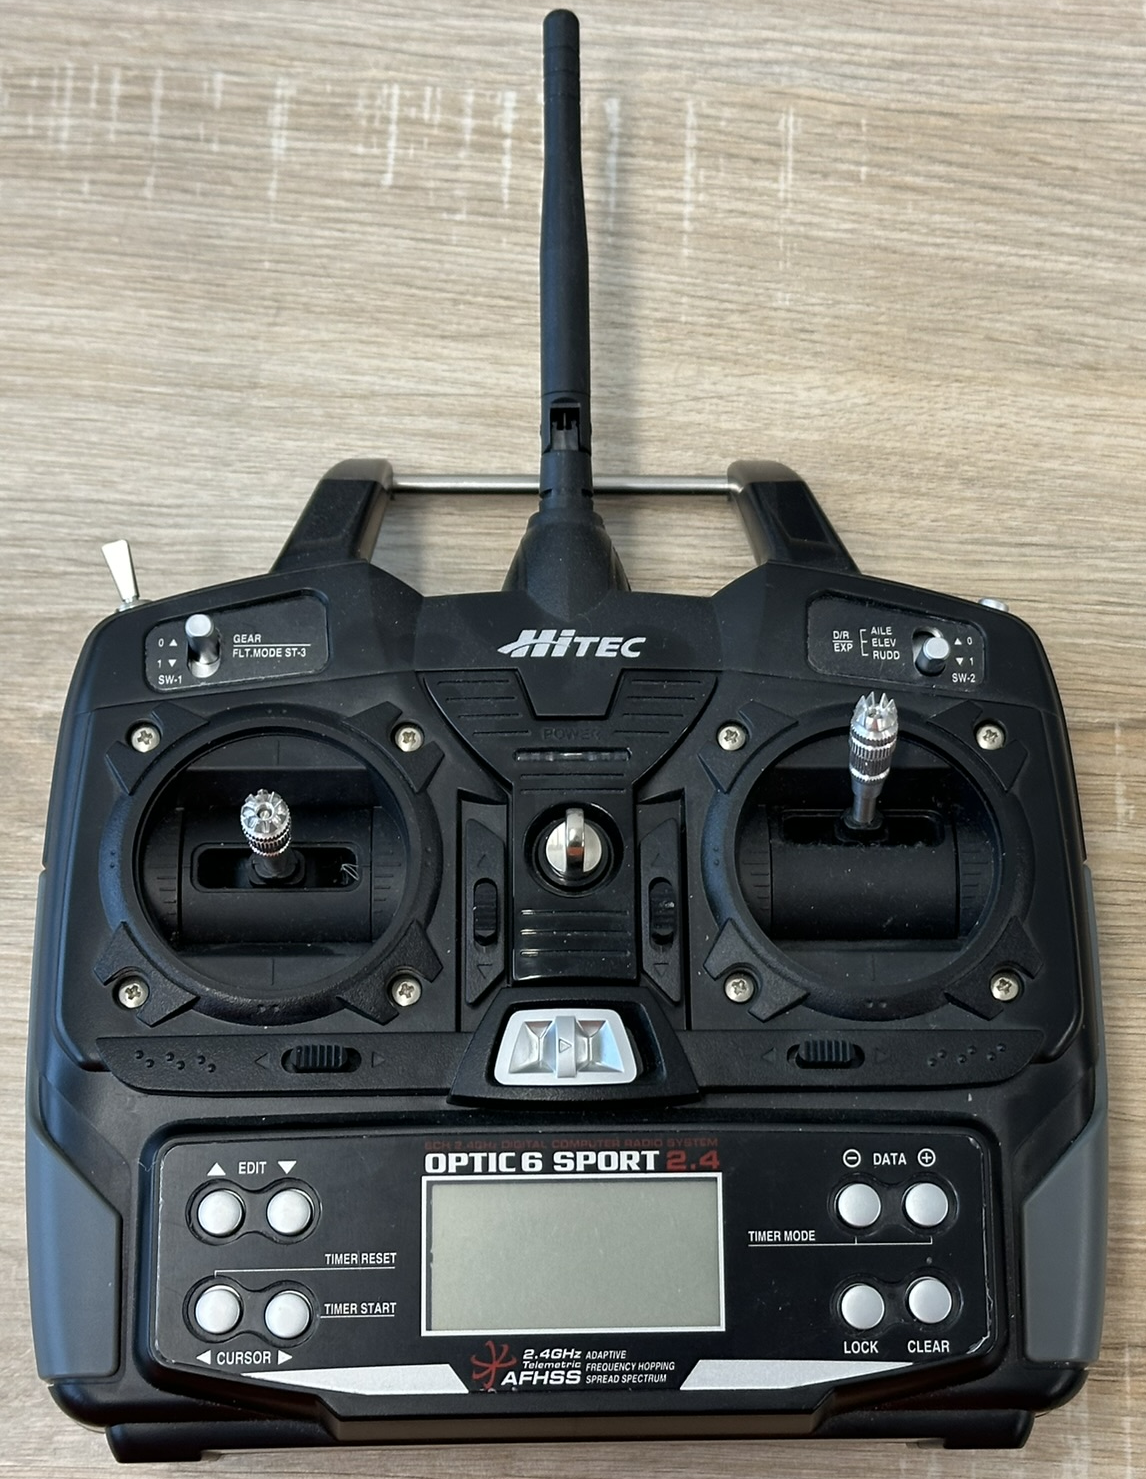
\includegraphics[width = .5\linewidth]{Figures/Joystick.png}
    \caption{Ovladač HITEC OPTIC 6 SPORT.}
    \label{fig:Joystick}
    \vspace{-10pt}
\end{figure}

\endinput
\chapter{Senzory}
\label{sec:Sensors}\

Platforma FRDM-K66F obsahuje tři senzory, které tvoří 9osou IMU jednotku.
NXP FXOS8700CQ slouží jako akcelerometr i~magnetometr a~NXP FXAS21002 jako gyroskop.
Tyto senzory komunikují s~platformou pomocí $I^2C$ \cite{frdmk66UserGuide}.

\section{Akcelerometr a~magnetometr}\

\textbf{NXP FXOS8700CQ} je pokročilý 6osý senzor, který kombinuje funkce 3osého
akcelerometru a~3osého magnetometru v~jednom čipu. Akcelerometr v~senzoru
FXOS8700CQ má nastavitelné rozsahy ±2 g, ±4 g, ±8 g s~14bitovým rozlišením, 
zatímco magnetometr poskytuje 16bitové rozlišení s~rozsahem ±1200 µT na osu. 
Pro komunikaci podporuje $I^2C$ a~$SPI$ rozhraní. Má dva piny pro~přerušení 
a~podporuje odesílat data rychlosti až 800 Hz pro každý senzor případně 400 Hz 
v~hybridním režimu. Tato integrace umožňuje zařízení zachytit komplexní 
data o~svém pohybu a~orientaci vůči zemskému gravitačnímu a~magnetickému poli. 
Orientace akcelerometru a~magnetometru je na~obrázku \ref{fig:FXOS_Orientation} 
\cite{FXOS8700CQ}.

\section{Gyroskop}\

\textbf{NXP FXAS21002} je vysoce výkonný 3osý senzor, který poskytuje 
data o~úhlové rychlosti zrychlení. Tento senzor má nastavitelné rozsahy 
±250, ±500, ±1000 a~±2000 stupňů za sekundu s~16bitovým rozlišením. 
Pro komunikaci podporuje $I^2C$ a~SPI rozhraní. Obsahuje dva piny pro~přerušení 
a~podporuje odesílat data rychlosti až 800 Hz, což umožňuje zařízení detekovat 
rotace kolem svých os. Orientace gyroskopu je zobrazena na obrázku 
\ref{fig:FXAS_Orientation} \cite{FXAS21002}.

\begin{figure}[ht]
    \centering
	\begin{subfigure}{0.35\textwidth}
	    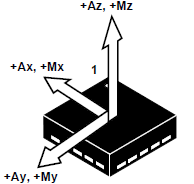
\includegraphics[width = \textwidth]{Figures/FXOS_Orientation.png}
        \label{fig:FXOS_Orientation}
        \caption{NXP FXOS8700CQ orientace \cite{FXOS8700CQ}.}
        \label{fig:FXOS_Orientation}
	\end{subfigure}
    \begin{subfigure}{0.35\textwidth}
        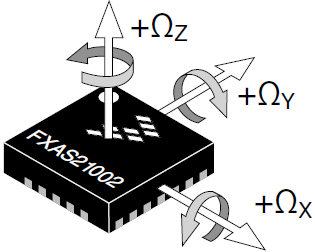
\includegraphics[width = \textwidth]{Figures/FXAS_Orientation.png}
        \label{fig:FXAS_Orientation}
         \caption{NXP FXAS21002 orientace \cite{FXAS21002}.}
         \label{fig:FXAS_Orientation}
    \end{subfigure}
	\caption{Orientace senzorů.}
\end{figure}

\section{Komunikace se senzory}\

Pro komunikaci se senzory je použita \textbf{$I^2C$ sběrnice}., která má 2
vodiče pro všechny zařízení, SDA a~SCL. \textbf{SDA} je datová linka, která
přenáší data mezi zařízeními, zatímco \textbf{SCL} je hodinová linka, která
synchronizuje přenos dat. Na sběrnici existuje jedno zařízení, které je
\textbf{master}, a~může komunikovat s~zařízeními, které jsou \textbf{slave}. Master
zařízení generuje hodinový signál a~určuje, kdy se data posílají a~přijímají. Každé
zařízení na sběrnici má svou vlastní adresu, která je 7 bitů dlouhá. Oba vodiče jsou
aktivní v~logické 0, což znamená, že v~klidovém stavu jsou oba vodiče v~logické 1.
Když je zařízení připojeno k~systému, musí být připojeno na zemi, aby mohlo
komunikovat \cite{I2C}.

Přenos na sběrnice vždy začíná START sekvencí a~končí STOP sekvencí, viz. obrázek
\ref{fig:I2C_FRAME}. Ty~jsou generovány master zařízením. \textbf{START} sekvence je
definovaná jako přechod z~logické 1 na~logickou 0 na SDA, zatímco na SCL je
v~logické 1. \textbf{STOP} sekvence oproti tomu má jako přechod z~logické~0
na~logickou 1 na SDA, zatímco na SCL je v~logické 1. Sběrnice je obsazena od začátku
START~sekvence až do konce STOP sekvence \cite{I2C}.

\begin{figure}[!h]
    \centering
    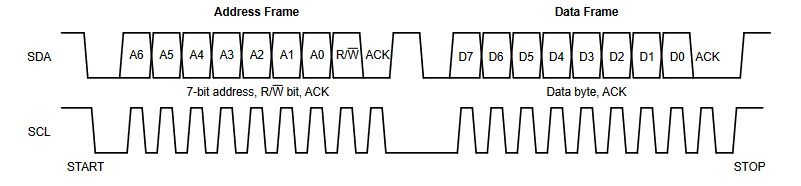
\includegraphics[width = .9\linewidth]{Figures/I2C_FRAME.png}
    \caption{$I^2C$ sběrnice \cite{I2C}.}
    \label{fig:I2C_FRAME}
\end{figure}

Pro zápis dat na sběrnici je nejprve nutné poslat adresu zařízení, které přijímá
data. Adresa má 7 bitů a~poslední bit je R/W, který určuje, zda se jedná o~zápis
nebo čtení. Poté jak slave pošle ACK bit (znamení, že je připraven přijmout data),
master posílá data a~slave potvrzuje přijetí ACK~bitem \cite{I2C}.

Čtení dat se podobá zápisu, po odeslání adresy zařízení, které posílá data, se
master přepne do~režimu čtení a~slave pošle data, která master potvrdí ACK
bitem \cite{I2C}.

\section{Konfigurace senzorů}\

Konfiguraci senzorů je probíhá posláním dat na jejich adresy. Adresy jsou \cite{frdmk66UserGuide}:
\begin{itemize}
    \item NXP FXOS8700CQ - 0x1D;
    \item NXP FXAS21002 - 0x21.
\end{itemize}

\subsection{Konfigurace NXP FXOS8700CQ}\

Pro nastavení NXP FXOS8700CQ bylo nastaveny následující registry: 

\begin{itemize}
    \item CTRL\_REG1 je použit pro přepnutí režimu senzoru mezi standby a~active.
    Pro jakékoliv změny v~registrech je nutné přepnout senzor do standby režimu.
    Pokud všechny registry byly nastaveny, je možné přepnout senzor do active
    režimu, a~dále tento registr použit pro nastavení frekvence vzorkování na 50 Hz
    a~zapnutí malého šumu \cite{FXOS8700CQ}.

    \item CTRL\_REG2 je použit pro zapnutí automatického režimu spanku, nízkého
    výkonu ve~spánku a~vysokého výkonu v~probuzení \cite{FXOS8700CQ}.

    \item CTRL\_REG4 je použit pro zapnutí data-ready přerušení \cite{FXOS8700CQ}.

    \item CTRL\_REG5 je použit pro nastavení pinu přerušení na INT2 \cite{FXOS8700CQ}.

    \item M\_CTRL\_REG1 je použit pro zapnutí hybridního režimu,jednorázového
    magnetického resetu a~nastavení oversample ratio na 7. V~hybridním režimu je
    možné získat data z~akcelerometru a~magnetometru současně \cite{FXOS8700CQ}.

    \item M\_CTRL\_REG2 je použit pro zapnutí automatického hybridního režimu
    inkrementu adresy. Co znamená, že po přečtení dat z~akcelerometru se začíná čist
    data z~magnetometru \cite{FXOS8700CQ}.

    \item Registr XYZ\_DATA\_CFG je použit pro nastavení rozsahu akcelerometru na ±4
    g \cite{FXOS8700CQ}.
\end{itemize}

Adresy a~hodnoty registrů jsou v~tabulce \ref{tab:FXOS8700CQ}.

\begin{table}[!h]
    \centering
	\begin{tabular}{ccc}
        \hline
        \textbf{Adresa} & \textbf{Registr} & \textbf{Hodnota} \\
        \hline
        0x2A            & CTRL\_REG1       & 0x1D             \\
        0x2B            & CTRL\_REG2       & 0x1E             \\
        0x2D            & CTRL\_REG4       & 0x01             \\
        0x2E            & CTRL\_REG5       & 0x00             \\
        0x5B            & M\_CTRL\_REG1    & 0x5F             \\
        0x5C            & M\_CTRL\_REG2    & 0x20             \\
        0x0E            & XYZ\_DATA\_CFG   & 0x01             \\
        \hline
    \end{tabular}
    \caption{Konfigurace NXP FXOS8700CQ.}
    \label{tab:FXOS8700CQ}
\end{table}

\subsection{Konfigurace NXP FXAS21002}\

Pro nastavení NXP FXAS21002 bylo nastaveny následující registry: 

\begin{itemize}
    \item CTRL\_REG0 je použit pro nastavení rozsahu gyroskopu na ±1000 stupňů za
    sekundu \cite{FXAS21002}.

    \item CTRL\_REG1 je použit pro přepnutí režimu senzoru mezi standby a~active.
    Pro jakékoliv změny v~registrech je nutné přepnout senzor do standby režimu.
    Pokud všechny registry byly nastaveny, je možné přepnout senzor do active
    režimu, a~dále tento registr použit pro nastavení frekvence vzorkování na 50
    Hz \cite{FXAS21002}.

    \item CTRL\_REG2 je použit pro zapnutí data-ready přerušení a~nastavení pinu
    přerušení na~INT1~\cite{FXAS21002}.
\end{itemize}

Adresy a~hodnoty registrů jsou v~tabulce \ref{tab:FXAS21002}.

\begin{table}[!h]
    \centering
    \begin{tabular}{ccc}
        \hline
        \textbf{Adresa} & \textbf{Registr} & \textbf{Hodnota} \\
        \hline
        0x0D            & CTRL\_REG0       & 0x01             \\
        0x13            & CTRL\_REG1       & 0x13             \\
        0x14            & CTRL\_REG2       & 0x0C             \\
        \hline
    \end{tabular}
    \caption{Konfigurace NXP FXAS21002.}
    \label{tab:FXAS21002}
\end{table}

\section{Čtení dat ze senzorů}\

Všechny senzory ukládají hodnoty do 6 registrů. Akcelerometr ukládá informace
o~naměřeném zrychlení do registrů 0x01 až 0x06. Gyroskop ukládá informace 
o~naměřeném úhlovém zrychlení do~registrů 0x01 až 0x06. Magnetometr ukládá 
informace o~naměřeném magnetickém poli do registrů 0x33 až 0x38. Zde jsou 
uložené data pro osy X, Y a~Z~\cite{FXAS21002}\cite{FXOS8700CQ}.

Obě zařízení umožňují číst data z~více registrů najednou. Pro získání dat stačí jen
začít čtení na první adrese datového registru 0x01. Data se posílají ve formátu big
endian, což znamená, že nejprve je poslán nejvyšší bajt a~poté nejnižší bajt \cite{FXAS21002}\cite{FXOS8700CQ}.

\section{Ukládání dat senzorů}\

V~momentě kdy senzor má data k~dispozici, vysílá signál přerušení. 
Signál přerušení se nazývá \uv{Data Ready} dle konfigurace senzorů. 

Senzor NXP FXAS21002 má povolené přerušení na GPIO pinu PTA29 
\cite{frdmk66UserGuide}. Tento pin je připojen do portu A. Přerušení na tomto portu bylo povolené a~priorita byla nastavěna na~2.

Senzor NXP FXOS8700CQ má povolené přerušení na GPIO pinu PTC13 
\cite{frdmk66UserGuide}. Tento pin je připojen do portu C. Přerušení na tomto portu bylo povolené a~priorita byla nastavěna na~2.

Jakmile je přijat signál přerušení, činnost procesoru je pozastavená. Následně se vykoná funkce spojená s~obsluhou přerušení. Takové obsluhy jsou dvě, pro port A~a~port C. 
První obsluha čte šest registru pro NXP FXAS21002 a~druhá 12 registru pro NXP 
FXOS8700CQ pomocí $I^2S$ sběrnice pro~získání dat ve všech třech osách. Tato data 
pak se ukládají do struktury Vec3, která obsahuje 3 osy x,y a~z~ve formátu 
int16\_t (16bitové číslo se znaménkem). Implementace obsluhy pro port A~je ve výpisu 
\ref{lst:interruptA} a~pro port C je \ref{lst:interruptC}.

\begin{lstlisting}[caption = Funkce obsluhy přerušení na portu A., label = lst:interruptA]
void PORTA_IRQHandler(void) {
    PORT_ClearPinsInterruptFlags(PORTA, 1U << 29);
    Shared::Vec3<int16_t> gyro;
    IMU& imu = core.getIMU();

    status_t status = I2C::readRegister(IMU::FXAS_ADDRESS, FXAS_OUT_X_MSB,
                                        fxasBuffer, sizeof(fxasBuffer));
    if (status == kStatus_Success) {
        gyro.x =
            static_cast<int16_t>(static_cast<uint16_t>(fxasBuffer[0] << 8) |
                                 static_cast<uint16_t>(fxasBuffer[1]));
        gyro.y =
            static_cast<int16_t>(static_cast<uint16_t>(fxasBuffer[2] << 8) |
                                 static_cast<uint16_t>(fxasBuffer[3]));
        gyro.z =
            static_cast<int16_t>(static_cast<uint16_t>(fxasBuffer[4] << 8) |
                                 static_cast<uint16_t>(fxasBuffer[5]));

        imu.setGyro(gyro);
    }
}
\end{lstlisting}

\begin{lstlisting}[caption = Funkce obsluhy přerušení na portu C., label = lst:interruptC]
void PORTC_IRQHandler(void) {
    PORT_ClearPinsInterruptFlags(PORTC, 1U << 13);
    Shared::Vec3<int16_t> accel, mag;
    IMU& imu = core.getIMU();

    status_t status = I2C::readRegister(IMU::FXOS_ADDRESS, FXOS_OUT_X_MSB,
                                        fxosBuffer, sizeof(fxosBuffer));
    if (status == kStatus_Success) {
        accel.x =
            static_cast<int16_t>(static_cast<uint16_t>(fxosBuffer[0] << 8) |
                                 static_cast<uint16_t>(fxosBuffer[1])) >>
            2;
        accel.y =
            static_cast<int16_t>(static_cast<uint16_t>(fxosBuffer[2] << 8) |
                                 static_cast<uint16_t>(fxosBuffer[3])) >>
            2;
        accel.z =
            static_cast<int16_t>(static_cast<uint16_t>(fxosBuffer[4] << 8) |
                                 static_cast<uint16_t>(fxosBuffer[5])) >>
            2;

        mag.x = static_cast<int16_t>(static_cast<uint16_t>(fxosBuffer[6] << 8) |
                                     static_cast<uint16_t>(fxosBuffer[7]));
        mag.y = static_cast<int16_t>(static_cast<uint16_t>(fxosBuffer[8] << 8) |
                                     static_cast<uint16_t>(fxosBuffer[9]));
        mag.z =
            static_cast<int16_t>(static_cast<uint16_t>(fxosBuffer[10] << 8) |
                                 static_cast<uint16_t>(fxosBuffer[11]));

        imu.setAccel(accel);
        imu.setMag(mag);
    }
\end{lstlisting}

\section{Výběr senzoru}\

Pro výběr vhodného senzoru byla analyzována data získaná po jízdě vozidla po dráze,
viz v~kapitole \ref{sec:PlatformControl}. Tato data jsou vizualizována na obrázku
\ref{fig:Sensors}.
\begin{figure}[!h]
    \centering
    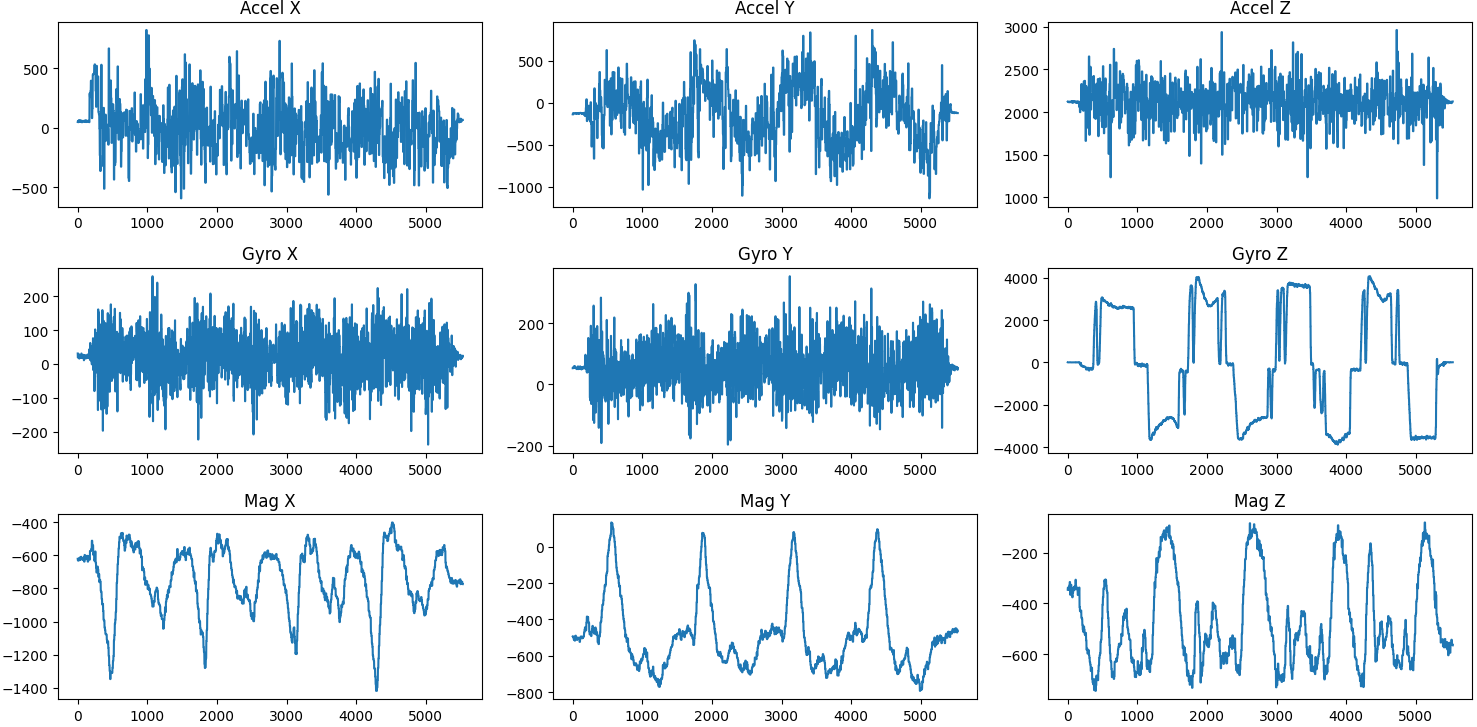
\includegraphics[width = 1\linewidth]{Figures/Sensors.png}
    \caption{Data ze senzorů.}
    \label{fig:Sensors}
\end{figure}

Z~obrázku je zřejmé, že otáčení vozidla koresponduje s~daty získanými
z~akcelerometru na ose $y$ a~gyroskopu na ose $z$. Nicméně je třeba poznamenat, 
že data z~akcelerometru obsahují významný šum, což vyžaduje implementaci vhodného
filtračního algoritmu před dalším zpracováním těchto dat. Dále je třeba zmínit, 
že data z~magnetometru nelze v~tomto případě využít, jelikož jsou negativně 
ovlivněna působením motorů vozidla. Přesunutí senzoru magnetometru na méně náchylné 
místo, například blíže ke kameře, by bylo ideální, avšak v~dané konfiguraci vozidla 
to není proveditelné. Vzhledem k~těmto omezením a~za účelem optimalizace rychlosti 
zpracování bude v~práci použita kombinace dat pouze z~akcelerometru a~gyroskopu.

\endinput
\chapter{Filtry}
\label{sec:Filters}\

Abychom odstranili šum je zapotřebí odfiltrovat signál. Tím se zásadně zlepší
detekce zatáčky. Tato kapitola je inspirovaná bakalářskou práce Šiguta Filipa
\uv{Krokoměr s~mikropočítačem ARM}~\cite{krokomer}. V~této práci byly popsány 
signálové filtry pro filtrování hodnot akcelerometru. Z~této práce byly použity 
filtry, které měly počet tiků menší než 200 za jedno volání filtrů. Tik představuje jeden cyklus časovače procesoru. Dále budou popsány FIR i~IIR filtry a~jejich porovnání.

\section{FIR filtry}\

\textbf{FIR filtry} jsou filtry s~konečnou impulzní odezvou. Tyto filtry používají
jen hodnoty ze vstupního signálu \cite{FIR}.

\subsection{Klouzavý průměr}\

\textbf{Klouzavý průměr} zprůměruje určitý počet hodnot ze vstupního signálu. Ve
tvaru rovnice to~bude:
\begin{equation}
y[i] = \frac{1}{M}\sum_{j = 0}^{M - 1}x[i+j],
\end{equation}
kde $y[\,\,]$ je výstupní hodnota, $M$ je počet hodnot a~$x[\,\,]$ je vstupní
hodnota \cite{Filters}.

Implementace tohoto filtru byla zjednodušena tím, že když hodnota součtu vstupních
hodnot se uloží, při výpočtu následující výstupní hodnoty se odečte vstupní hodnota
posledního vzorku a~přičte se hodnota nového vzorku. Výsledná hodnota se pak vydělí
hodnotou $M$ \cite{krokomer}.

Při filtrování signálu byla po experimentech zvolena hodnota $M$ = 8.

\section{IIR filtry}\

\textbf{IIR filtry} jsou filtry s~nekonečnou impulzní odezvou. Tyto filtry, 
na rozdíl od FIR filtrů, používají mechanizmus zpětné vazby, tzn. výstupní
hodnoty \cite{IIR}.

Všechny implementované IIR filtry jsou ve tvaru:
\begin{equation}
y[n] = \sum_{i = 0}^{j}a_{i}x[n - i] + \sum_{i = 1}^{k}b_{i}y[n - i],
\end{equation}
kde $y$ je výstupní hodnota, $x$ je vstupní hodnota a~$a_i$ i~$b_i$ jsou
koeficienty.

\subsection{Jednopólová dolní propust}\

Filtr má jen dva koeficienty:
\begin{align}
\begin{split}
a_0 &= 1 - x \\
b_1 &= x
\end{split}
\end{align}
kde $x$ je hodnota v~intervalu <0; 1>, která kontroluje silu filtru \cite{Filters}.

Zvolená hodnota $x$ je 0,85. Z~toho plynou hodnoty koeficientu $a_0 = 0,15$ 
a~$b_1 = 0,85$.

\subsection{Čtyřstupňová dolní propust}\

Filtr obsahuje 5 koeficientů:
\begin{align}
\begin{split}
a_0 &= (1 - x)^4 \\
b_1 &= 4x \\
b_2 &= -6x^2 \\
b_3 &= 4x^3 \\
b_4 &= -x^4
\end{split}
\end{align}
kde $x$ je hodnota v~intervalu <0; 1>, která kontroluje silu filtru \cite{Filters}.

Zvolená hodnota $x$ je 0,6.

\subsection{Dvoupólový Čebyševův filtr}\

Filtr obsahuje 5 koeficientů. Tyto koeficienty jsou z~tabulky hodnot pro dvoupólový
Čebyševův filtr pro frekvence $f_c = 0,075$ \cite{Filters}:
\begin{align}
\begin{split}
a_0 &= 3,869430E-02f \\
a_1 &= 7,738860E-02f \\
a_2 &= 3,869430E-02f \\
b_1 &= 1,392667E+00f \\
b_2 &= -5,474446E-01 \\
\end{split}
\end{align}

\section{Testování}\

Všechny filtry byly testovány pomocí algoritmu, který byl popsán v~kapitole
\ref{sec:PlatformControl}. Obrázky \ref{fig:NoFilter} a~\ref{fig:filters} zobrazují
původní nefiltrovány signál a~výstupy jednotlivých filtrů aplikovaných na tento
signál.

Po analýze výsledků jsem dospěl k~závěru, že nejlepší výsledky ukazují filtry
\uv{Jednopólová dolní propust} a~\uv{Čtyřstupňová dolní propust}. První zmíněný byl 
použit pro implementaci kvůli lepší redukce šumu.

\begin{figure}[!h]
	\centering
    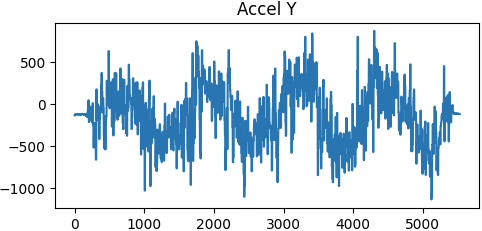
\includegraphics[width = 0.7\linewidth]{Figures/NoFilter.png}
    \caption{Nefiltrovaný signál.}
    \label{fig:NoFilter}
\end{figure}

\begin{figure}[!h]
    \centering
        \subfloat[Klouzavý průměr.]{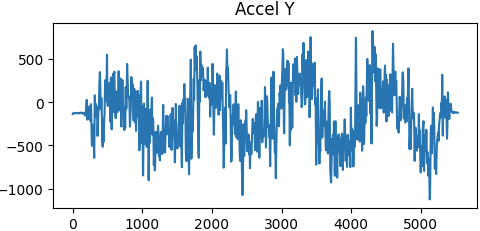
\includegraphics[width = .5\textwidth]{Figures/MovingAverage.png}\label{fig:MovingAverage}}
	    \subfloat[Jednopólová dolní propust.]{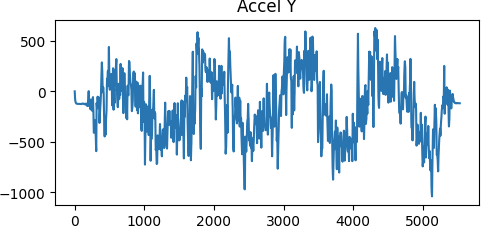
\includegraphics[width = .5\textwidth]{Figures/SinglePole.png}\label{fig:SinglePole}} \\
        \subfloat[Čtyřstupňová dolní propust.]{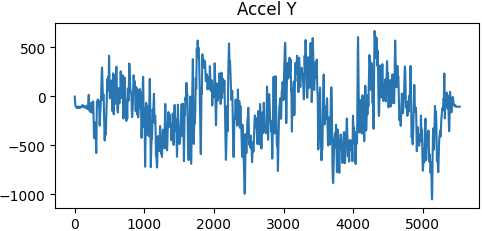
\includegraphics[width = .5\textwidth]{Figures/FourStage.png}\label{fig:FourStage}}
    	\subfloat[Dvoupólový Čebyševův filtr.]{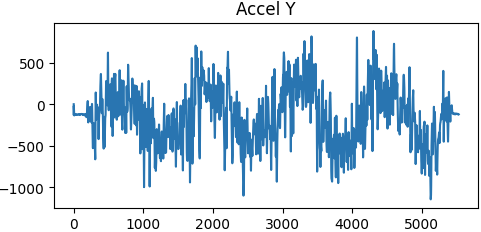
\includegraphics[width = .5\textwidth]{Figures/Chebyshev.png}\label{fig:Chebyshev}}
    \caption{Ukázky aplikovaných filtrů.}
    \label{fig:filters}
\end{figure}

\endinput


\printbibliography[title={Seznam použité literatury}]
\addcontentsline{toc}{chapter}{Seznam použité literatury}
\end{document}
